\documentclass[11pt]{article}
%Gummi|063|=)
\title{\textbf{Algorithms I -- supervision 3}}
\author{James Wood}
\usepackage{listings}
\usepackage{bold-extra}
\usepackage{xcolor}
\usepackage{amsmath}
\usepackage{enumitem}
\usepackage{tikz}
\usetikzlibrary{arrows}
%\ifx\pdftexversion\undefined
%\usepackage[dvips]{graphicx}
%\else
%\usepackage[pdftex]{graphicx}
%\DeclareGraphicsRule{*}{mps}{*}{}
%\fi

\lstset{
  basicstyle=\small,
  basewidth=0.5em,
  frame=single,
  breaklines=true,
  %postbreak=\raisebox{0ex}[0ex][0ex]{
  %  \ensuremath{\color{red}\hookrightarrow\space}
  %}
  language=python,
  literate=
    {<=}{{\(\leq\)}}1
    {>=}{{\(\geq\)}}1
    {&&}{{\(\wedge\)}}1
    {||}{{\(\vee\)}}1
    {->}{{\(\rightarrow\)}}1
}

\tikzset{
  treenode/.style = {align=center, inner sep=0pt, text centered,
    font=\sffamily},
  bnode/.style = {treenode, circle, white, draw=black,
    fill=black, text width=1.5em},
  rnode/.style = {treenode, circle, red, draw=red,
    text width=1.5em, very thick},
  leaf/.style = {treenode, rectangle, draw=black,
    minimum width=0.5em, minimum height=0.5em}
}

\begin{document}
\renewcommand{\labelenumi}{(\alph{enumi})}
\renewcommand{\labelenumii}{(\roman{enumii})}

\maketitle

\section{Postfix notation}
\begin{lstlisting}
def infixToPostfix(ts):
    # Assume that `ts' is a list of tokens,
    # and that we can distinguish numbers from operators.

    # Table of precedence:
    # (   | 0
    # + - | 1
    # * / | 2
    # All left associating

    for t in ts:
        if t is '(':
            push(t, stack)
        else if t is ')':
            while head(stack) is not '(':
                append(pop(stack), output)
            pop(stack)
        else if t is a number:
            append(t, output)
        else if t is an operator:
            while (nonEmpty(stack) &&
                   precedence(t) <= precedence(head(stack))):
                append(pop(stack), output)
            push(t, stack)

    while nonEmpty(stack):
        append(pop(stack), output)

    return output
\end{lstlisting}
Analysis by the potential method (with the size of the stack corresponding to potential cost) shows that input of a '(' has cost 2, input of a ')' has cost 0, input of a number has cost 1 and input of an operator has cost 1. All of these have constant cost, so the algorithm runs in linear time.

Going in the reverse direction, producing a correct infix expression would be simple, but producing a correct infix expression with a minimal number of brackets would be more difficult.

\section{Binary search trees}
\begin{enumerate}
\item Consider:

  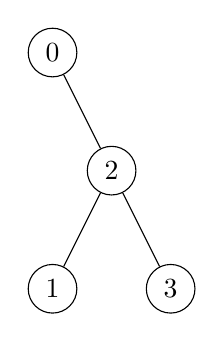
\begin{tikzpicture}
    \node[circle,draw](z){0}
    child[missing]{}
    child{
      node[circle,draw]{2}
      child{node[circle,draw]{1}}
      child{node[circle,draw]{3}}
    };
  \end{tikzpicture}

  A search for 3 yeilds \(A=\{1\}\), \(B=\{0,2,3\}\) and \(C=\{\}\). Picking \(a=1\) and \(b=0\) contradicts the conjecture.

  Technically, when \(C\) is empty, \(\forall a\in A,b\in B,c\in C.a\leq b\wedge b\leq c\) is vacuously true, so we instead take a search for 4 in

  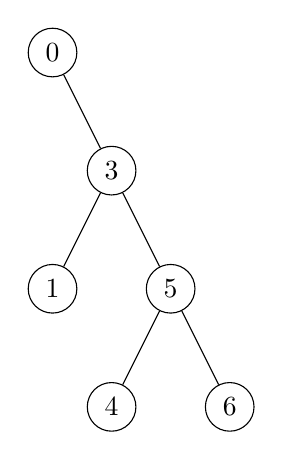
\begin{tikzpicture}
    \node[circle,draw](z){0}
    child[missing]{}
    child{
      node[circle,draw]{3}
      child{node[circle,draw]{1}}
      child{
        node[circle,draw]{5}
        child{node[circle,draw]{4}}
        child{node[circle,draw]{6}}
      }
    };
  \end{tikzpicture}

  to be a counterexample.
\item By the algorithm for finding the successor, the successor of a node with a right child is the leftmost node in its right subtree. If the successor had a left child, that child would be left of the successor and be in all of the subtrees the successor is in, contradicting the fact that the successor is leftmost in the right subtree.
\item
  \begin{minipage}[t]{\linewidth}
    \begin{lstlisting}
data Direction = Up | DownLeft | DownRight
# Maybe type (and Functor instance) from Haskell

def pathBetween(n, o):
    # n is the current node and o is the target node.
    # Nodes are aware of their parent
    # and whether they are a left or right child.

    def pathFrom(p, q):
        if p == q:
            Just []
        else if key(p) > key(q):
            Nothing
        else:
            upPath = map((Up ::),pathFrom(parent(p), q))
                       if isLeftChild(p) else Nothing
            upPath if isJust(upPath) else
                       map((DownRight ::),pathFrom(right(p), q))

    def reversePath(path):
        def f(ps, qs):
            case qs:
                []             : ps
                Up        :: ds: f(DownLeft :: ps, ds)
                DownRight :: ds: f(Up :: ps, ds)
        f([], path)

    if key(n) <= key(o):
        fromJust(pathFrom(n, o))
    else:
        reversePath(fromJust(pathFrom(o, n)))
    \end{lstlisting}
  \end{minipage}
\end{enumerate}

\section{Red-black trees}
\begin{enumerate}
\item Construct a red-black tree such that the leftmost path contains alternating black and red nodes, and all nodes outside this path are black. A tree of height \(2\cdot k+2\) can be produced from a tree of height \(2\cdot k+1\) by adding a red node to the end of the leftmost path. A tree of height \(2\cdot k+1\) can be produced from a tree of height \(2\cdot k\) by adding two black nodes to each external node and adding a black node to the penultimate black node in the leftmost path. Any right subtrees are perfect, so have \(2^i-1\) nodes, where \(i\) is its height. For trees of height \(2\cdot k\), the minimum number of nodes is \(\sum_{i\in[0..k)}2\cdot\left( 1+2^i-1 \right)\), which is equal to \(2\cdot\left( 2^k-1 \right)\). For a tree of height \(2\cdot k+1\), we derive from this the minimum \(2\cdot\left( 2^{k+1}-1 \right)-1\), which is equal to \(2^{k+2}-3\), by removing a red node from the tree of height \(2\cdot k+2\).

  A red-black tree with a maximal number of nodes will be perfect, and thus contain \(2^h-1\) nodes.
\item
  2-node \([a]\):

  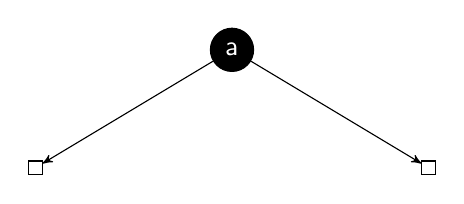
\begin{tikzpicture}[->,>=stealth',level/.style={sibling distance = 5cm/#1,level distance = 1.5cm}]
    \node[bnode]{a}
    child{node[leaf]{}}
    child{node[leaf]{}}
    ;
  \end{tikzpicture}

  3-node \([a,b]\)

  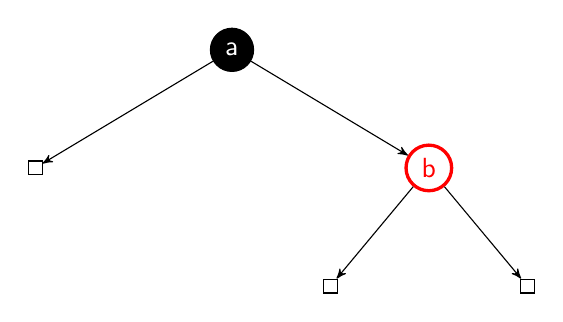
\begin{tikzpicture}[->,>=stealth',level/.style={sibling distance = 5cm/#1,level distance = 1.5cm}]
    \node[bnode]{a}
    child{node[leaf]{}}
    child{
      node[rnode]{b}
      child{node[leaf]{}}
      child{node[leaf]{}}
    }
    ;
  \end{tikzpicture}

  4-node \([a,b,c]\)

  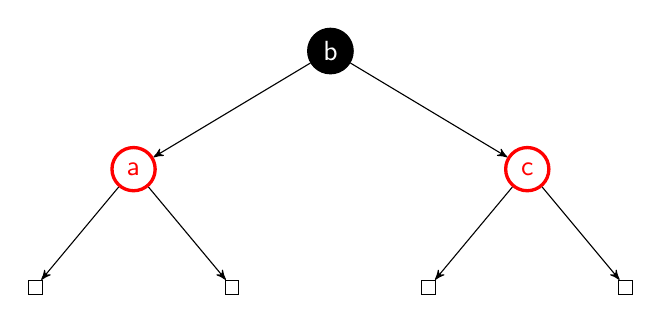
\begin{tikzpicture}[->,>=stealth',level/.style={sibling distance = 5cm/#1,level distance = 1.5cm}]
    \node[bnode]{b}
    child{
      node[rnode]{a}
      child{node[leaf]{}}
      child{node[leaf]{}}
    }
    child{
      node[rnode]{c}
      child{node[leaf]{}}
      child{node[leaf]{}}
    }
    ;
  \end{tikzpicture}
\end{enumerate}

\section{Hash tables}
\begin{enumerate}
\item
  \begin{tabular}[t]{r || l | l | l}
    hash & \multicolumn{3}{|c}{values} \\
    \hline
    0 & 20 & 8  & 10 \\
    1 & 19 & 11 & \\
    2 & 12 &    & \\
    3 & 23 &    & \\
    4 &    &    & \\
    5 & 15 &    & \\
    6 &    &    & \\
    7 & 7  & 17 & \\
  \end{tabular}
\item The value stored at that location can be hashed and compared against the hash of the value being searched for.
\item If the naïve approach of simply removing the entry is taken, any values appearing later in the same overspill will become inaccessible, as the algorithm for finding them will stop as soon as it finds the null value. Instead, we need to find the last item in the overspill and put it in the place of the deleted item.
\end{enumerate}

\section{Binomial heap}
\begin{enumerate}
\item Let \(f\,n\) be the number of nodes in an order-\(n\) binomial tree. It is defined by \(f\,0=1\) and \(f\,(1+n)=2\cdot f\,n\). Obviously, \(f\,n=2^n\), so the sequence \(\mathrm{map}\,f\,[0..k)\) gives the place values for a \(k\) bit binary representation of a number.
\item Start with the trees of lowest order and do binary addition. If either place is empty, use the other place's tree. When both places have a tree, merge them as follows and add the result onto the next column. To merge two trees of equal order, compare their heads and, in the case of a minheap, add the larger head's tree as a subtree of the smaller head. Given that each column's merging takes constant time, the algorithm runs in logarithmic time on the number of items, since there are approximately \(\log_2n\) bits in the binary representation of \(n\).
\end{enumerate}

\section{Stacks and queues}
\begin{enumerate}
\item One stack represents the first part of the queue, with the front of the queue accessible, and the other stack represents the second part of the queue with the back of the queue accessible. Enqueueing is done by pushing to the back stack. Dequeueing is done by popping from the front stack. If the front stack is empty, pop all of the elements off the back stack and push them to the front stack. Using the potential method, where the potential is the length of the back stack, enqueueing costs \(1+1\) (operation plus increase in potential) and dequeueing costs either \(1\) (if the front stack is non-empty) or \(1+n-n\) (popping and pushing everything takes \(n\), but \(n\) potential is removed). All of these costs are constant, so each operation has linear amortized cost.
\item To push, enqueue the element to the first queue. To pop, dequeue every element from the first queue, except the last, into the second queue. Dequeue the last element and output it. Then, swap the roles of the two queues. Again using the potential method, with potential being the length of the first queue, pushing has cost \(2\) and popping has cost \(n\). This gives quadratic amortized performance.
\end{enumerate}

\end{document}